\section{0x34\ 数学\ 初等数论-质数}
\label{sec:0x34a}

\subsection{质数}

\Highlight{质数}：若一个正整数 $n$ ($n > 1$) 无法被除了 $1$ 和它自身以外的任何正整数整除，则称该数为质数（或素数）。否则称该数为合数。特别地，$1$ 既不是质数也不是合数。

\Highlight{质数分布函数}：$\pi(n)$ 表示 $1 \sim n$ 中的质数个数。当 $n$ 足够大时，$\pi(n) \sim \frac{n}{\ln n}$。

\Highlight{\textbf{唯一分解定理}}：任意一个大于 $1$ 的正整数 $n$，都可以唯一分解成有限个质数的乘积，记作
\[
n = p_1^{c_1}p_2^{c_2}\dots p_t^{c_t}
\]
其中 $p_i$ 均为质数且满足 $p_1 < p_2 < \dots < p_t$，$c_i$ 均为正整数。

\Highlight{质因数的根号分治}：一个正整数 $n$，大于 $\sqrt{n}$ 的质因子最多只有 $1$ 个。

\subsubsection{阶乘的质因数分解}

对于阶乘 $n! = 1 \times 2 \times \dots \times n$，由于每一项均为 $[1, n]$ 中的正整数，故分解出的质因数也均为 $[1, n]$ 中的质数。

筛出 $1 \sim n$ 中的所有质数，\textbf{对于每个质数 $p$，考虑 $n!$ 中一共包含了多少个质因子 $p$}。

共有大约 $\frac{n}{\ln n}$ 个质数，每个质数 $p$ 的求解需要 $\log_p n$ 的开销，故时间复杂度 $\mathcal{O}(n)$。

\Highlight{阶乘 $n!$ 中包含质数 $p$ 的次数}：
\[
\sum_{i = 1}^{\lfloor \log_p n \rfloor} \left\lfloor \frac{n}{p^i} \right\rfloor
\]
简单推导：设 $c_i$ 表示 $i$ 包含的质因子 $p$ 个数，则阶乘 $n!$ 包含 $p$ 的个数为 $\sum_{j = 1}^{\infty} \sum_{i = 1}^n j[c_i = j]$，进一步得 $\sum_{j = 1}^{\infty}\sum_{i = 1}^n [c_i \geq j]$，不难发现其中 $\sum_{i = 1}^n [c_i \geq j] = \left\lfloor \frac{n}{p^j} \right\rfloor$。

\Highlight{阶乘 $n!$ 中包含合数 $m$ 的次数}：将 $m$ 唯一分解成 $m = p_1^{c_1}p_2^{c_2}\dots p_t^{c_t}$ 的形式。

记 $v_p(n) = \sum_{i = 1}^{\lfloor \log_p n \rfloor} \left\lfloor \frac{n}{p^i} \right\rfloor$，答案为
\[
\min_{1 \leq i \leq t} \left\lfloor \frac{v_{p_i}(n)}{c_i} \right\rfloor
\]

\subsubsection{埃氏筛}

注意到，任意整数 $x$ ($x > 1$) 的倍数 $2x, 3x, \dots$ 都不是质数。

从 $2$ 到 $n$ 依次扫描每一个数 $x$，若 $x$ 尚未被标记，则说明 $x$ 为质数，并且将其倍数 $2x, 3x, \dots, \left\lfloor \frac{n}{x} \right\rfloor x$ 均标记为合数。

时间复杂度 $\mathcal{O}(n \log \log n)$。

在开 O2 优化的情况下，\texttt{std::bitset} 连续读写效率较高，可以加以优化埃氏筛。

\begin{quoteblock}
埃氏筛的时间复杂度证明：\textbf{相当于是证明 $1 \sim n$ 中所有质数的倒数之和为 $\mathcal{O}(\log \log n)$ 级别}。

由质数分布函数，可以推测第 $n$ 个质数的大小为 $\Theta(n \log n)$，于是有
\[
\begin{aligned}
\sum_{k = 1}^{\pi(n)} \frac{1}{p_k} & = \mathcal{O}\left( \sum_{k = 2}^{\pi(n)} \frac{1}{k \log k} \right) \\
& = \mathcal{O}\left(\int_2^{\pi(n)} \frac{1}{x \log x} \mathrm{dx} \right) \\
& = \mathcal{O}(\log \log \pi(n)) \\
& = \mathcal{O}(\log \log n)
\end{aligned}
\]
\end{quoteblock}

\InputCode{cpp}{contents/0x30 数学/code/0x34 埃氏筛.cpp}

\subsubsection{线性筛}

为了避免埃氏筛重复标记合数。在线性筛中，我们希望确定一个合数的方式能够唯一。

从 $2$ 到 $n$ 依次扫描每一个数 $x$，在标记合数时，\textbf{我们只在 $x$ 的基础上乘一个质因子 $p$，并且保证 $p$ 是 $xp$ 的最小质因子}。这样做，每个合数只会被自己的最小质因子标记一次。并且顺带还能筛出每个数的最小质因子。

时间复杂度 $\mathcal{O}(n)$。

由于线性筛每次只扩展一个最小质因子的结构，可以额外处理很多信息（例如筛出积性函数）。

\InputCode{cpp}{contents/0x30 数学/code/0x34 线性筛.cpp}

\subsection{狄利克雷前缀和}

\Highlight{狄利克雷前缀和}：已知 $a_1, \dots, a_n$，求出 $b_1, \dots, b_n$，其中 $b_i = \sum_{j \mid i} a_j$。

记 $j = \prod p_k^{\alpha_k}, i = \prod p_k^{\beta_k}$，则 $a_j$ 对 $b_i$ 有贡献当且仅当：对于所有的 $k$ 均有 $\alpha_k \leq \beta_k$。类似地，运用\textbf{高维前缀和}即可。

\begin{minted}{cpp}
// 注意：要先枚举质数 prime[j]
for (int j = 1; j <= primeCount; j ++) {
    for (int i = 1; i <= n / prime[j]; i ++) {
        f[i * prime[j]] += f[i];
    }
}
\end{minted}

\Highlight{狄利克雷后缀和}：已知 $a_1, \dots, a_n$，求出 $b_1, \dots, b_n$，其中 $b_i = \sum_{i \mid j} a_j$。

\begin{minted}{cpp}
// 注意：要先枚举质数 prime[j]
for (int j = 1; j <= primeCount; j ++) {
    for (int i = n / prime[j]; i >= 1; i --) {
        f[i] += f[i * prime[j]];
    }
}
\end{minted}

\Highlight{狄利克雷倒前缀和}：已知 $b_1, \dots, b_n$，反推 $a_1, \dots, a_n$，其中 $b_i = \sum_{j \mid i} a_j$。

\begin{minted}{cpp}
// 注意：要先枚举质数 prime[j]
for (int j = 1; j <= primeCount; j ++) {
    for (int i = n / prime[j]; i >= 1; i --) { // 顺序与正变换相反
        f[i * prime[j]] -= f[i];
    }
}
\end{minted}

\Highlight{狄利克雷倒后缀和}：已知 $b_1, \dots, b_n$，反推 $a_1, \dots, a_n$，其中 $b_i = \sum_{i \mid j} a_j$。

\begin{minted}{cpp}
// 注意：要先枚举质数 prime[j]
for (int j = 1; j <= primeCount; j ++) {
    for (int i = 1; i <= n / prime[j]; i ++) { // 顺序与正变换相反
        f[i] -= f[i * prime[j]];
    }
}
\end{minted}

\subsection{Miller-Rabin 素性测试}

回顾一些内容：

\Highlight{费马小定理}：设 $p$ 是素数，对于任意整数 $a$（$a$ 不能是 $p$ 的倍数），满足 $a^{p - 1} \equiv 1 \pmod p$。

\Highlight{Fermat 伪素数}：若满足 $a^{n - 1} \equiv 1 \pmod n$，但 $n$ 不是素数，则称 $n$ 为以 $a$ 为底的 Fermat 伪素数。

\textbf{对于任何固定的基底 $a$，都存在无穷多个的 Fermat 伪素数}。

\Highlight{Fermat 素性测试}：不断地选取在 $[2, n - 1]$ 中的基底 $a$，并检验是否每次都满足 $a^{n - 1} \equiv 1\pmod n$。

\textbf{即使检查了所有与 $n$ 互质的基底 $a$，依然无法保证 $n$ 是素数}。这样的数 $n$ 称为 Carmichael 数，有无穷多个。

\Highlight{二次探测定理}：设 $p$ 是奇素数，则同余方程 $x^2 \equiv 1 \pmod p$ 的解为 $x \equiv 1 \pmod p$ 或 $x \equiv p - 1\pmod p$。

\Separator{}

\Highlight{Miller-Rabin 素性测试}：Miller-Rabin 素性测试，结合了费马小定理和二次探测定理，是一种概率性素性测试（可以放心使用）。

先将 $a^{n - 1} \equiv 1 \pmod n$ 中的指数 $n - 1$，分解成 $n - 1 = u \times 2^t$ 的形式。

每次随机一个基底 $a$，进行如下的判断：

\begin{itemize}
\item 先使用快速幂求出 $v = a^u \bmod n$。如果 $v = 1$ 或 $v = n - 1$，则该轮测试通过。
\item 然后对这个值进行 $t - 1$ 次平方操作，途中如果该值等于 $n - 1$，则该轮测试通过。
\item 否则该轮测试不通过。
\end{itemize}

在不考虑乘法的开销时，对 $n$ 进行 $k$ 轮测试的时间复杂度为 $\mathcal{O}(k \log n)$。

可以证明，奇合数 $n$ ($n > 9$) 通过随机选取的一个基底的概率不超过 $\frac{1}{4}$。\textbf{因此随机选取 $k$ 个基底后，仍然误判的概率不超过 $\frac{1}{4^k}$}。随机选取 $10$ 次较为保险。

对于 $[2, 2^{64})$ 范围内的数，工业上通常选用 $\{ 2, 325, 9375, 28178, 450775, 9780504, 1795265022 \}$ 作为检验的基底。为了方便也可以选择前 $12$ 个质数作为基底。

\subsection{Pollard-Rho 质因数分解}

\Highlight{Pollard-Rho}：用于找出合数 $n$ 的某一个非平凡因数 $d$（非平凡因数：非 $1$ 且非 $n$ 的因数）。

若一个正整数 $n$ 为合数，那么 $n$ 的最小质因子 $p$ 满足 $p \leq \sqrt{n}$。

如果随机生成 $\mathcal{O}(\sqrt{p})$ 个正整数，由生日悖论，可能存在两个正整数 $a, b$ 满足 $a \equiv b \pmod p$，此时 $|a - b|$ 是 $p$ 的倍数，于是查询 $\gcd(|a - b|, n)$ 即可得到 $n$ 的一个因子。

\begin{quoteblock}
生日悖论：在 $[1, n]$ 中随机选择正整数，选出两个相同数的期望轮数为 $\mathcal{O}(\sqrt{n})$ 级别（近似 $\sqrt{\frac{\pi n}{2}}$）。
\end{quoteblock}

但这样做，枚举数对的时间复杂度还是太高。

记映射 $f(x) = (x^2 + c) \bmod n$，其中 $c$ 是一个随机选取的常数（$c \neq 0, -2$）。Pollard 构造了这样的一个伪随机序列 $\{x_i\}$，满足 $x_i = f(x_{i - 1})$。

考虑序列 $\{ x_i \bmod p \}$，由于 $x_i$ 仅仅与 $x_{i - 1}$ 有关，且 $x_i \bmod p \in [0, p)$，\textbf{所以 $\{ x_i \bmod p \}$ 是一个混循环序列}。

建图后形似 $\rho$ 形（rho），\textbf{由生日悖论可得尾长与环长均为 $\mathcal{O}(\sqrt{p})$ 级别}。

% 原 HTML：<img src="https://cdn.luogu.com.cn/upload/image_hosting/tw7xcqnu.png" style="zoom:50%;" />
\begin{center}
\noindent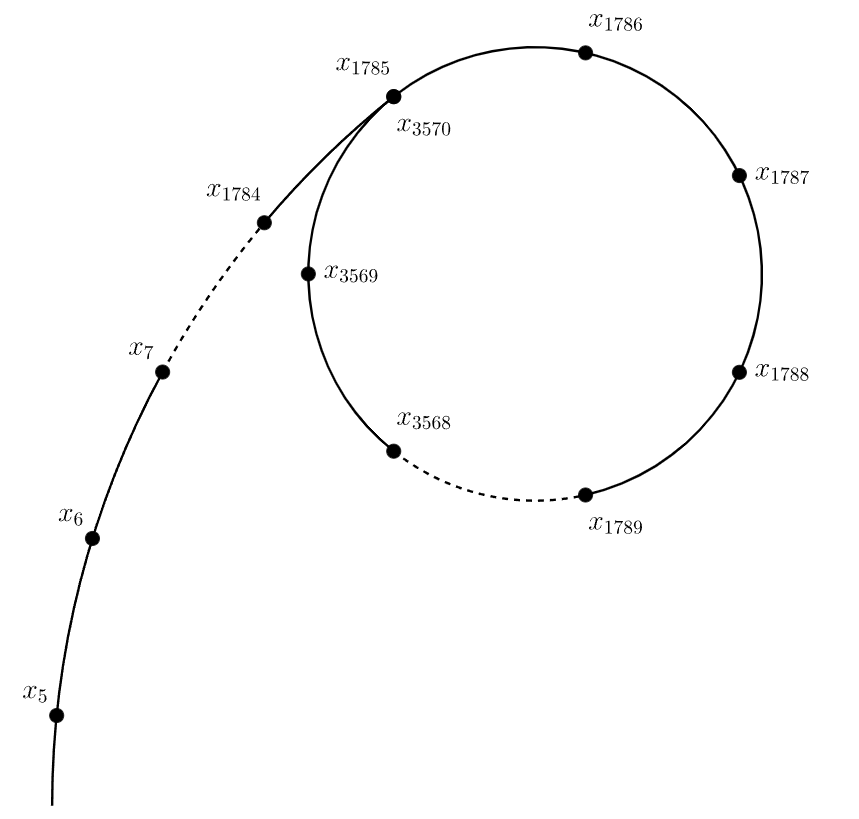
\includegraphics[width=0.6\textwidth]{contents/0x30 数学/figures/0x34 rho 形图.png}
\end{center}

我们发现，\textbf{若 $x \equiv y \pmod p$，必有 $f(x) \equiv f(y) \pmod p$}。由此可得\textbf{在模 $p$ 的环上，只要某个相距 $d$ 步的点对满足条件，则所有相距 $d$ 步的点对均满足条件}。所以我们每次最好要检查不同的距离。

\textbf{Brent 倍增迭代}：初始有两个点 $a, b$，在第 $k$ 轮，$a$ 原地不动，$b$ 不断地向前共计 $2^k$ 步，最后再让 $a$ 直接跳到 $b$ 的位置。$b$ 的每一步移动，我们都计算 $d = \gcd(|a - b|, n)$，当第一次出现 $d > 1$ 时

\begin{itemize}
\item 若 $1 < d < n$，则我们已经找到了一个非平凡因数，直接返回 $d$。
\item 若 $d = n$，则说明我们已经完整地跑完了一个环，继续在环上跑也没有意义。\newline{}
此时我们应该换个映射，或者换一个初始值继续做。
\end{itemize}

\textbf{进一步，我们想要降低求解 $\gcd$ 的次数}。注意到，如果 $\gcd(a, n) > 1$，则对于任意正整数 $b$ 均有 $\gcd(ab \bmod n, n) = \gcd(ab, n) > 1$。

也就是说，如果 $\gcd\left(\prod |x_i - x_j| \bmod n, n\right) > 1$，那么其中必有一对 $x_i, x_j$ 满足 $\gcd(|x_i - x_j|, n) > 1$。

于是我们每 $k$ 对 $a, b$ 就计算一次 $\gcd$。时间复杂度 $\mathcal{O}(\sqrt{p} + k^{-1}\sqrt{p} \log n)$，当 $k$ 与 $\log n$ 大致相等时，\textbf{可以得到 $\mathcal{O}(\sqrt{p})$ 的理论复杂度}。具体实现中，一般取 $k = 128$。

\Highlight{Pollard-Rho 质因数分解}：如果要对 $n$ 进行质因数分解，先使用 Miller-Rabin 判断 $n$ 是否是质数，若 $n$ 为合数，则使用 Pollard-Rho 找出 $n$ 的一个非平凡因数 $d$，得到两个规模分别为 $d$ 和 $\frac{n}{d}$ 的两个子问题，递归进行求解。

\InputCode{cpp}{contents/0x30 数学/code/0x34 素性测试与质因数分解（Miller-Rabin + Pollard-Rho）.cpp}

\section{0x34\ 数学\ 初等数论-约数}
\label{sec:0x34b}

\subsection{约数}

\Highlight{整除}：设 $d, n \in \mathbb{Z}$ 且 $d \neq 0$，如果 $\exists q \in \mathbb{Z}$ 使得 $qd = n$，那么称 $d$ 整除 $n$（记作 $d \mid n$）。

\Highlight{整除的简单性质}：

\begin{itemize}
\item $a \mid b \land b \mid c \Longrightarrow a\mid c$。
\item $a \mid b \land a \mid c \Longrightarrow \forall x, y \in \mathbb{Z}, a \mid (xb + yc)$。
\item 设 $m \neq 0$，则 $a \mid b \Longrightarrow ma \mid mb$。
\item 设 $\gcd(a, m) = 1$，则 $a \mid mb \Longrightarrow a\mid b$。
\end{itemize}

\Highlight{约数个数}：

\begin{itemize}
\item $n$ 的约数个数必定不超过 $2\sqrt{n}$。实际上很难到达该上界，可以简单认为在 $10^6 \sim 10^{18}$ 范围内为 $\mathcal{O}(\sqrt[3]{n})$ 级别。
\item $1\sim n$ 的约数个数总和为 $\mathcal{O}(n \log n)$ 级别。
\end{itemize}

\subsection{最大公约数与最小公倍数}

\Highlight{最大公约数}：最大的公共约数（\textbf{G}reatest \textbf{C}ommon \textbf{D}ivisor，简写 GCD）。

\Highlight{最小公倍数}：最小的公共倍数（\textbf{L}east \textbf{C}ommon \textbf{M}ultiple，简写 LCM）。

\Highlight{\textbf{唯一分解角度下的 gcd 与 lcm}}：设 $a = p_1^{c_1}p_2^{c_2}\dots$，$b = p_1^{d_1}p_2^{d_2} \dots$，则有
\[
\begin{gathered}
\gcd(a, b) = p_1^{\min(c_1, d_1)}p_2^{\min(c_2, d_2)} \dots \\
\mathrm{lcm}(a, b) = p_1^{\max(c_1, d_1)}p_2^{\max(c_2, d_2)} \dots
\end{gathered}
\]
在唯一分解角度下，\textbf{gcd 相当于是对每个指数取 min，lcm 相当于是对每个指数取 max}。

\Highlight{gcd 的简单性质}：

\begin{itemize}
\item $\gcd(a_1, \dots, a_n) = \gcd(|a_1|, \dots, |a_n|)$。
\item $\gcd(a, 0) = \gcd(a, a) = |a|$。
\item $\gcd(bq + r, b) = \gcd(r, b)$。
\item 设 $\gcd(a, m) = 1$，则 $\gcd(a, mb) = \gcd(a, b)$。
\item $\gcd(ma_1, \dots, ma_n) = |m| \gcd(a_1, \dots, a_n)$。
\end{itemize}

\Highlight{lcm 的简单性质}：

\begin{itemize}
\item $\mathrm{lcm}(a_1, \dots, a_n) = \mathrm{lcm}(|a_1|, \dots, |a_n|)$。
\item $\mathrm{lcm}(a, 1) = \mathrm{lcm}(a, a) = |a|$。
\item $\mathrm{lcm}(ma_1, \dots, ma_n) = |m| \operatorname{lcm}(a_1, \dots, a_n)$。
\end{itemize}

\subsubsection{gcd 和 lcm 的常见恒等式}

\Highlight{gcd-lcm 恒等式}：
\[
\gcd(a, b) \operatorname{lcm}(a, b) = ab
\]
请注意！\textbf{该式子扩展到三元以上几乎不成立！}

事实上当 $n \geq 3$ 时，$\gcd(a_1, \dots, a_n) \operatorname{lcm}(a_1, \dots, a_n) = a_1\dots a_n$ 当且仅当 $a_1, \dots, a_n$ 两两互质。

\Highlight{gcd 和 lcm 的结合律}：
\[
\begin{gathered}
\gcd(a, b, c) = \gcd(\gcd(a, b), c) \\
\mathrm{lcm}(a, b, c) = \mathrm{lcm}(\mathrm{lcm}(a, b), c)
\end{gathered}
\]
该式子扩展到任意多元仍然成立。

于是可以使用恒等式 $\mathrm{lcm}(a, b) = \frac{ab}{\gcd(a, b)}$，用来求解 $\mathrm{lcm}(a, b, c)$，以及 $\mathrm{lcm}(a_1, \dots, a_n)$。

\Highlight{gcd 对乘法的分配律}：
\[
\gcd(a, bc) = \gcd(a, b) \gcd\left(\frac{a}{\gcd(a, b)}, c\right)
\]
根据对乘法的分配律计算 $\gcd(a, b_1\dots b_n)$。每次处理 $b_i$ 时，计算 $t = \gcd(a, b_i)$，然后将 $a$ 除以 $t$（相当于是将已计算的质因数贡献去掉），答案乘以 $t$。

\Highlight{gcd 的差分律}：
\[
\gcd(a_1, a_2, \dots, a_n) = \gcd(a_1, a_2 - a_1, \dots, a_n - a_{n - 1})
\]
通过差分律，我们可以维护差分数组的 gcd，以实现 “区间加” 与 “区间 gcd”。

\Highlight{斐波那契数列 gcd 恒等式}：
\[
\gcd(\mathrm{Fib}_n, \mathrm{Fib}_m) = \mathrm{Fib}_{\gcd(n, m)}
\]
\Highlight{幂差 gcd 恒等式}：\textbf{不妨设 $a \geq b$，当 $\gcd(a, b) = 1$ 时}，有
\[
\gcd(a^n - b^n, a^m - b^m) = a^{\gcd(n, m)} - b^{\gcd(n, m)}
\]
简单推导：

\textbf{右边整除左边}：可以证明 $x - y \mid x^k - y^k$。

\begin{quoteblock}
$k$ 次方差公式：$x^k - y^k = (x - y)(x^{k - 1} + x^{k - 2}y + \dots + xy^{k - 2} + y^{k - 1})$。
\end{quoteblock}

对于 $n, m$ 的公约数 $d$ 来说，可以证得 $a^d - b^d \mid a^n - b^n$ 与 $a^d - b^d \mid a^m - b^m$。

于是 $a^d - b^d \mid \gcd(a^n - b^n, a^m - b^m)$。所以
\[
a^{\gcd(n, m)} - b^{\gcd(n, m)} \mid \gcd(a^n - b^n, a^m - b^m)
\]
\textbf{左边整除右边}：

\begin{quoteblock}
“降幂引理”：不妨设 $r \geq s$，当 $\gcd(a, b) = 1$ 时，有
\[
\gcd(a^r - b^r, a^s - b^s) \mid a^{r - s} - b^{r - s}
\]

证明：设 $d$ 为 $a^r - b^r, a^s - b^s$ 的公约数。

因为 $(a^r - b^r) - a^{r - s}(a^s - b^s) = b^s(a^{r - s} - b^{r - s})$，可以证得 $d \mid b^s(a^{r - s} - b^{r - s})$；同理可得 $d \mid a^s(a^{r - s} - b^{r - s})$。

又由于 $\gcd(a, b) = 1$，于是 $d \mid a^{r - s} - b^{r - s}$，“降幂引理” 得证。
\end{quoteblock}

对 $\gcd(a^n - b^n, a^m - b^m)$ 反复应用 “降幂引理”，过程等价于辗转相除法。所以
\[
\gcd(a^n - b^n, a^m - b^m) \mid a^{\gcd(n, m)} - b^{\gcd(n, m)}
\]

\subsection{最大公约数常见求法}

已有的轮子：\texttt{std::gcd(a, b)}。

\subsubsection{求法 1：辗转相除法}

（也称之为欧几里得算法）

对于 $\forall a, b \in \mathbb{N}$ 且 $b \neq 0$，有
\[
\gcd(a, b) = \gcd(b, a \bmod b)
\]

\begin{itemize}
\item 当 $a < b$ 时，一次迭代后就会转化为 $a \geq b$。
\item 当 $a \geq b$ 时，由于 $a \bmod b \leq \frac{a}{2}$，这样的迭代不超过 $\log_2 a$ 次。
\end{itemize}

时间复杂度 $\mathcal{O}(\log \max(a, b))$。

使用辗转相除法求解斐波那契数列相邻两项的 gcd，会让该算法达到最坏复杂度。

\begin{minted}{cpp}
// 辗转相除法
int gcd(int a, int b) {
    return b == 0 ? a : gcd(b, a % b);
}
\end{minted}

\subsubsection{求法 2：更相减损术}

对于 $\forall a, b \in \mathbb{N}$，不妨设 $a\geq b$，有
\[
\begin{gathered}
\gcd(a, b) = \gcd(a, a - b) = \gcd(b, a - b) \\
\gcd(2a, 2b) = 2\gcd(a, b)
\end{gathered}
\]

\begin{itemize}
\item 当 $a = b$ 时，$\gcd(a, b) = a$。
\item “两个偶数”：$\gcd(a, b) = 2\gcd(\frac{a}{2}, \frac{b}{2})$。
\item “一奇一偶”：不妨设 $a$ 为偶数，$\gcd(a, b) = \gcd(\frac{a}{2}, b)$。
\item “两个奇数”：不妨设 $a \geq b$，$\gcd(a, b) = \gcd(a - b, b)$。
\end{itemize}

当至少有一个偶数的时候，每次迭代至少会将 $a, b$ 之一减半。而两个奇数相减会得到偶数。

时间复杂度 $\mathcal{O}(\log \max(a, b))$。

更相减损术常用于计算高精度 gcd（因为“高精度取模”复杂度较高，“高精度减法”以及“高精除低精”复杂度较低）。

\InputCode{cpp}{contents/0x30 数学/code/0x34 gcd（更相减损术）.cpp}

\subsubsection{求法 3：递推}

初值 $\gcd(i, 0) = \gcd(0, i) = i$，递推式 $\gcd(i, j) = \gcd(i - j, j)$。

时间复杂度：预处理 $\mathcal{O}(n^2)$，查询 $\mathcal{O}(1)$。

\begin{minted}{cpp}
for (int i = 0; i <= n; i ++) {
    g[i][0] = g[0][i] = i;
    for (int j = 1; j <= i; j ++) {
        g[i][j] = g[j][i] = g[i - j][j];
    }
}
\end{minted}

\subsubsection{求法 4：基于值域预处理的快速 gcd}

\textbf{引理}：对于任意正整数 $n$，一定可以被拆分成三个正整数 $a, b, c$ ($a \leq b \leq c$) 的乘积，其中 $a, b\leq \sqrt{n}$，且 $c \leq \sqrt{n}$ 与 $c \in \mathbb{P}$ 至少有一个成立。

\textbf{证明 1}：假设 $c > \sqrt{n}$ 且 $c \notin \mathbb{P}$。因为 $c > \sqrt{n}$ 且 $abc = n$，所以 $ab \leq \sqrt{n}$。由于 $c$ 不是质数，设 $c = xy$，显然 $x, y$ 不可能同时 $>\sqrt{n}$，不妨设 $x \leq y$，则必有 $x \leq \sqrt{n}$。此时 $n$ 可以被拆分成 $x, ab, y$ 的乘积。不断对 $y$ 进行相同的讨论。

由于数值不断递减，迭代到最后 $c \leq \sqrt{n}$ 与 $c \in \mathbb{P}$ 至少有一个成立。

\textbf{证明 2}：考虑归纳。当 $n = 1$ 时显然成立。当 $n > 1$ 时，设 $p$ 为 $n$ 的最小质因数，设 $a', b', c'$ ($a' \leq b' \leq c'$) 为 $\frac{n}{p}$ 的一组合法拆分。

\begin{itemize}
\item 当 $p \leq \sqrt[4]{n}$ 时。由于 $a' \leq \sqrt[3]{\frac{n}{p}}$，所以 $pa' \leq \sqrt[3]{np^2} \leq \sqrt{n}$。此时 $pa', b', c'$ 为一组合法拆分。
\item 当 $p > \sqrt[4]{n}$ 时。假设 $a' \geq p$，则 $n = pa'b'c' \geq p^4 > n$ 矛盾，故 $a' < p$。由于 $p$ 为 $n$ 的最小质因数，所以 $a' = 1$。此时 $p, b', c'$ 为一组合法拆分。
\end{itemize}

\Separator{}

预处理：通过线性筛得出 $1 \sim n$ 所有数的最小质因数。然后根据证明 2，递推得出 $1 \sim n$ 所有数的合法拆分。对于 $i > 1$，设 $p$ 为 $i$ 的最小质因数，\textbf{将 $\frac{i}{p}$ 的合法拆分中的最小数乘以 $p$ 即可得到 $i$ 的合法拆分}。最后预处理出所有 $0 \leq x, y \leq \sqrt{n}$ 的 $\gcd(x, y)$。

查询：当询问 $\gcd(p, q)$ 时，根据 gcd 对乘法的分配律，依次考虑 $q$ 的合法拆分 $a, b, c$，设当前考虑到的数为 $x$。

\begin{itemize}
\item 计算 $t = \gcd(p, x)$，具体地：
  \begin{itemize}
  \item 若 $x$ 为合数（此时 $x \leq \sqrt{n}$），则 $\gcd(p, x) = \gcd(x, p \bmod x)$。使用预处理的 gcd 值回答即可。
  \item 若 $x$ 为质数，则当且仅当 $p$ 为 $x$ 的倍数时 $\gcd(p, x) = x$，否则 $\gcd(p, x) = 1$。
  \end{itemize}
\item 然后将 $p$ 除以 $t$，答案乘以 $t$。
\end{itemize}

时间复杂度：预处理 $\mathcal{O}(n)$，查询 $\mathcal{O}(1)$。

\InputCode{cpp}{contents/0x30 数学/code/0x34 gcd（基于值域预处理的快速 gcd）.cpp}

\subsection{类欧几里得算法}

\Highlight{类欧几里得算法}：用来解决一类形如 $\left\lfloor \frac{ai + b}{c} \right\rfloor$ 结构的求和问题。

基本模型为
\[
f(a, b, c, n) = \sum_{i = 0}^n \left\lfloor \frac{ai + b}{c} \right\rfloor
\]
首先，可以转化为 $0 \leq a, b < c$ 的情况
\[
\begin{aligned}
f(a, b, c, n) & = \sum_{i = 0}^n \left\lfloor \frac{ai + b}{c} \right\rfloor \\
& = \sum_{i = 0}^n \left\lfloor \frac{\left(\left\lfloor \frac{a}{c} \right\rfloor c + (a \bmod c) \right)i + \left(\left\lfloor \frac{b}{c} \right\rfloor c + (b \bmod c)\right)}{c} \right\rfloor \\
& = \sum_{i = 0}^n \left( \left\lfloor \frac{a}{c} \right\rfloor i + \left\lfloor \frac{b}{c} \right\rfloor + \left\lfloor \frac{(a \bmod c) i + (b \bmod c)}{c} \right\rfloor \right) \\
& = \frac{n(n + 1)}{2} \left\lfloor \frac{a}{c} \right\rfloor + (n + 1)\left\lfloor \frac{b}{c} \right\rfloor + f(a \bmod c, b \bmod c, c, n)
\end{aligned}
\]
然后，令 $m = \left\lfloor \frac{an + b}{c} \right\rfloor$
\[
\begin{aligned}
f(a, b, c, n) & = \sum_{i = 0}^n \left\lfloor \frac{ai + b}{c} \right\rfloor \\
& = \sum_{i = 0}^n \sum_{j = 0}^{m - 1} \left[ j < \left\lfloor \frac{ai + b}{c} \right\rfloor \right] \\
& = \sum_{i = 0}^n \sum_{j = 0}^{m - 1} \left[ j + 1 \leq \frac{ai + b}{c} \right] \\
& = \sum_{i = 0}^n \sum_{j = 0}^{m - 1} \left[ cj + c - b - 1 < ai \right] \\
& = \sum_{j = 0}^{m - 1} \sum_{i = 0}^n \left[ \left\lfloor \frac{cj + c - b - 1}{a} \right\rfloor < i \right] \\
& = \sum_{j = 0}^{m - 1} \left( n - \left\lfloor \frac{cj + c - b - 1}{a} \right\rfloor \right) \\
& = nm - f(c, c - b - 1, a, m - 1)
\end{aligned}
\]

结合这两步操作，二元组 $(a, c) \to (c, a \bmod c)$，相当于对 $(a, c)$ 进行辗转相除法，故称之为类欧几里得算法。

时间复杂度 $\mathcal{O}(\log \min(a, c))$。

\InputCode{cpp}{contents/0x30 数学/code/0x34 类欧几里得算法.cpp}

\section{0x34\ 数学\ 初等数论-取整}
\label{sec:0x34c}

\subsection{取整}

\Highlight{向下取整}：$\lfloor x \rfloor$，表示不超过 $x$ 的最大整数（floor）。

\Highlight{向上取整}：$\lceil x \rceil$，表示不小于 $x$ 的最小整数（ceiling）。

注意：C++ 中的整数除法结果\textbf{向零取整}，取模结果\textbf{与被除数同号}，与数学中的取整有较大区别。

\Highlight{取整的简单性质}：

\begin{itemize}
\item $x - 1 < \lfloor x \rfloor \leq x$，$x \leq \lceil x \rceil < x + 1$。
\item $\lfloor -x \rfloor = - \lceil x \rceil$，$\lceil -x \rceil = - \lfloor x \rfloor$。
\end{itemize}

\subsubsection{取整的常见恒等式}

\Highlight{上下取整的相互转化}：$n, m \in \mathbb{Z}$，$m > 0$
\[
\begin{gathered}
\left\lceil \frac{n}{m} \right\rceil = \left\lfloor \frac{n + m - 1}{m} \right\rfloor = \left\lfloor \frac{n - 1}{m} \right\rfloor + 1 \\
\left\lfloor \frac{n}{m} \right\rfloor = \left\lceil \frac{n - m + 1}{m} \right\rceil = \left\lceil \frac{n + 1}{m} \right\rceil - 1
\end{gathered}
\]
\Highlight{上下取整的嵌套恒等式}：$a, b, c \in \mathbb{N}_+$
\[
\begin{gathered}
\left\lfloor \frac{ \left\lfloor \frac{a}{b} \right\rfloor }{c} \right\rfloor = \left\lfloor \frac{a}{bc} \right\rfloor \\
\left\lceil \frac{ \left\lceil \frac{a}{b} \right\rceil }{c} \right\rceil = \left\lceil \frac{a}{bc} \right\rceil
\end{gathered}
\]

\Highlight{上下取整对加法的恒等式}：$A, B, C, D \in \mathbb{N}_+$
\[
\begin{gathered}
\left\lfloor \frac{ \left\lfloor \frac{A}{B} \right\rfloor + C }{D} \right\rfloor = \left\lfloor \frac{A + BC}{BD} \right\rfloor \\
\left\lceil \frac{ \left\lceil \frac{A}{B} \right\rceil + C }{D} \right\rceil = \left\lceil \frac{A + BC}{BD} \right\rceil
\end{gathered}
\]

\subsection{数论分块}

也称之为整除分块。

\subsubsection{下取整数论分块}

给出一个正整数 $n$，记 $D_n$ 表示 $\left\lfloor \frac{n}{d} \right\rfloor$ 所有可能的取值构成的集合，即 $D_n = \{ \left\lfloor \frac{n}{d} \right\rfloor \mid 1 \leq d \leq n \}$。

\textbf{性质 1}：$\left\lfloor \frac{n}{d} \right\rfloor$ 的取值不超过 $2\sqrt{n}$ 种，即 $|D_n| \leq 2\sqrt{n}$。

简单推导：

\begin{itemize}
\item 当 $d \leq \sqrt{n}$ 时，因为 $d$ 的取值不超过 $\sqrt{n}$ 种，所以此时 $\left\lfloor \frac{n}{d} \right\rfloor$ 的取值不超过 $\sqrt{n}$ 种。
\item 当 $d > \sqrt{n}$ 时，因为 $\left\lfloor \frac{n}{d} \right\rfloor \leq \sqrt{n}$，所以此时 $\left\lfloor \frac{n}{d} \right\rfloor$ 的取值不超过 $\sqrt{n}$ 种。
\end{itemize}

\textbf{性质 2}：若 $m \in D_n$，则 $D_m \subseteq D_n$。

简单推导：设 $m = \left\lfloor \frac{n}{k} \right\rfloor$，此时对于任意 $d \in \mathbb{N}_+$
\[
\left\lfloor \frac{m}{d} \right\rfloor = \left\lfloor \frac{\left\lfloor \frac{n}{k} \right\rfloor}{d} \right\rfloor = \left\lfloor \frac{n}{kd} \right\rfloor \in D_n
\]
这意味着，\textbf{如果我们想要递归地应用数论分块（类似杜教筛）}，在计算过程中涉及到的取值集合均为 $D_n$。

\Highlight{下取整数论分块}：快速地划分出 $\left\lfloor \frac{n}{d} \right\rfloor$ 取值相同的所有区间。

由于函数 $\frac{n}{x}$ 在区间 $(0, +\infty)$ 上单调递减，所以 $\left\lfloor \frac{n}{x} \right\rfloor$ 取值相同的所有自变量 $x$ \textbf{构成一段连续的区间}。并且由上述分析，这样的区间不超过 $2\sqrt{n}$ 个。

对于任意 $i$ ($1 \leq i \leq n$)，需要找到一个最大的 $j$ ($i \leq j \leq n$) 满足 $\left\lfloor \frac{n}{i} \right\rfloor = \left\lfloor \frac{n}{j} \right\rfloor$。由不等式 $\left\lfloor \frac{n}{i} \right\rfloor \leq \frac{n}{j}$ 可得 $\boldsymbol{j = \left\lfloor \frac{n}{\left\lfloor \frac{n}{i} \right\rfloor} \right\rfloor}$。

根据该公式，我们就可以根据区间的左端点计算出右端点。于是依次遍历所有区间即可。

\begin{minted}{cpp}
// h 表示 x 的上界
for (int x = 1, nx; x <= h; x = nx + 1) {
    nx = h;
    if (x <= n) {
        chmin(nx, n / (n / x));
    }
    // 区间 [x, nx] 内：下取整的值均为 n/x
}
\end{minted}

\begin{quoteblock}
By the way：数论分块套数论分块的时间复杂度为 $\mathcal{O}(n^{\frac{3}{4}})$。
\end{quoteblock}

\subsubsection{上取整数论分块}

\Highlight{上取整数论分块}：快速地找出 $\lceil \frac{n}{d} \rceil$ 取值相同的所有区间。

由恒等式 $\left\lceil \frac{n}{m} \right\rceil = \left\lfloor \frac{n - 1}{m} \right\rfloor + 1$ 可知，$n$ 的上取整数论分块与 $n - 1$ 的下取整数论分块，分出的区间是一样的。

于是套用 $n - 1$ 的下取整数论分块即可，\textbf{注意 $d \geq n$ 的特殊情况}。

\begin{minted}{cpp}
// h 表示 x 的上界
for (int x = 1, nx; x <= h; x = nx + 1) {
    nx = h;
    if (x < n) {
        chmin(nx, (n - 1) / ((n - 1) / x));
    }
    // 区间 [x, nx] 内：上取整的值均为 (n-1)/x+1
}
\end{minted}

\subsubsection{多维数论分块}

\Highlight{二维数论分块}：快速地找出 $\left\lfloor \frac{n}{d} \right\rfloor, \left\lfloor \frac{m}{d} \right\rfloor$ 取值均相同的所有区间。

显然，这样的区间不超过 $2\sqrt{n} + 2\sqrt{m}$ 个。

对于任意 $i$，需要找到一个最大的 $j$ 满足 $\left\lfloor \frac{n}{i} \right\rfloor = \left\lfloor \frac{n}{j} \right\rfloor, \left\lfloor \frac{m}{i} \right\rfloor = \left\lfloor \frac{m}{j} \right\rfloor$。则有 $\boldsymbol{j = \min\left\{ \left\lfloor \frac{n}{ \left\lfloor \frac{n}{i} \right\rfloor } \right\rfloor, \left\lfloor \frac{m}{ \left\lfloor \frac{m}{i} \right\rfloor } \right\rfloor \right\}}$。

扩展到多维也是一样。

\begin{minted}{cpp}
// h 表示 x 的上界
for (int x = 1, nx; x <= h; x = nx + 1) {
    nx = h;
    if (x <= n) {
        chmin(nx, n / (n / x));
    }
    if (x <= m) {
        chmin(nx, m / (m / x));
    }
    // 区间 [x, nx] 内：n, m 对 x 下取整的值分别为 n/x, m/x
}
\end{minted}

\subsection{积性函数与狄利克雷卷积}

\Highlight{积性函数}：若数论函数 $f(n)$，对于\textbf{任意互质}正整数 $x, y$，都有 $f(xy) = f(x)f(y)$，则称 $f(n)$ 为积性函数。

\Highlight{完全积性函数}：若数论函数 $f(n)$，对于\textbf{任意}正整数 $x, y$，都有 $f(xy) = f(x)f(y)$，则称 $f(n)$ 为完全积性函数。

\Highlight{积性函数的简单性质}：

\begin{itemize}
\item 对于任意积性函数 $f(x)$（除了恒为 $0$ 的函数），有 $f(1) = 1$。
\item 对于任意积性函数 $f(x), g(x)$，\textbf{以下的函数仍为积性函数}
\[
\begin{gathered}
f(x^p) \\
f^p(x) \\
f(x)g(x) \\
\sum_{d \mid x} f(d)g\left( \frac{x}{d} \right)
\end{gathered}
\]

\item 对于任意积性函数 $f(x)$，将 $x$ 唯一分解成 $x = p_1^{c_1}p_2^{c_2}\dots p_t^{c_t}$，有 $f(x) = \prod_{i = 1}^t f(p_i^{c_i})$。
\end{itemize}

\subsubsection{常见积性函数（及性质）}

\paragraph{单位函数（完全积性）}
\[
\epsilon(n) = [n = 1]
\]

\paragraph{恒等函数（完全积性）}
\[
\mathrm{ID}_k(n) = n^k
\]

当 $k = 1$ 时，亦可简写为 $\mathrm{ID}(n) = n$。

\paragraph{常数函数（完全积性）}
\[
1(n) = 1
\]

\paragraph{约数函数（积性）}

\Highlight{约数函数}：
\[
\sigma_k(n) = \sum_{d \mid n} d^k
\]

当 $k = 0$ 时，$\sigma_0(n)$ 表示 $n$ 的约数个数函数。

\Highlight{约数个数函数的前缀和}：
\[
\sum_{i = 1}^n \sigma_0(i) = \sum_{i = 1}^n \left\lfloor \frac{n}{i} \right\rfloor
\]
\Highlight{乘积的约数个数函数}：
\[
\begin{gathered}
\sigma_0(ij) = \sum_{x \mid i} \sum_{y \mid j} [\gcd(x, y) = 1] \\
\sigma_0(ijk) = \sum_{a \mid i} \sum_{b \mid j} \sum_{c \mid k} [\gcd(a, b) = \gcd(b, c) = \gcd(a, c) = 1]
\end{gathered}
\]
简单推导（仅证二维）：从唯一分解的角度，对每个质因子 $p$ 单独考虑。$p$ 在 $(x, y)$ 中的出现情况数，为 $i, j$ 中质因子 $p$ 的个数之和再加 $1$。将所有质因子 $p$ 的贡献相乘，这正是 $\sigma_0(ij)$ 的表达式。

可以扩展至更多维。

\paragraph{欧拉函数（积性）}

\Highlight{欧拉函数}：$\varphi(n)$，表示 $1 \sim n$ 中与 $n$ 互质的数的个数。将 $n$ 唯一分解成 $n = p_1^{c_1}p_2^{c_2}\dots p_t^{c_t}$，则欧拉函数为
\[
\varphi(n) = n \prod_{i = 1}^t (1 - \frac{1}{p_i})
\]

\Highlight{乘积的欧拉函数}：
\[
\varphi(ij) = \frac{\varphi(i) \varphi(j) \gcd(i, j)}{\varphi(\gcd(i, j))}
\]
简单推导：设 $P(n)$ 表示 $n$ 的质因数集合，则有 $P(ij) = P(i) \cup P(j)$ 与 $P(\gcd(i, j)) = P(i) \cap P(j)$。

由容斥原理得
\[
\prod_{p \mid ij} \left(1 - \frac{1}{p}\right) = \frac{\prod_{p \mid i} \left(1 - \frac{1}{p}\right) \prod_{p \mid j} \left(1 - \frac{1}{p}\right)}{\prod_{p \mid \gcd(i, j)} \left(1 - \frac{1}{p}\right)}
\iff
\frac{\varphi(ij)}{ij} = \frac{ \frac{\varphi(i)}{i} \frac{\varphi(j)}{j} }{\frac{\varphi(\gcd(i, j))}{\gcd(i, j)}}
\]

\paragraph{莫比乌斯函数（积性）}

\Highlight{莫比乌斯函数}：$\mu(n)$，将 $n$ 唯一分解成 $n = p_1^{c_1}p_2^{c_2}\dots p_t^{c_t}$，则莫比乌斯函数有如下的定义
\[
\mu(n) = \begin{cases}
(-1)^t & \forall i\in[1, t], c_i = 1 \\
0 & \exists i\in[1, t], c_i > 1
\end{cases}
\]
特别地，$\mu(1) = 1$。

\Highlight{莫比乌斯函数的平方}：
\[
\mu^2(n) = \sum_{d^2 \mid n} \mu(d)
\]
简单推导：记 $m = \prod p_i^{\left\lfloor c_i / 2 \right\rfloor}$，则 $d^2 \mid n \iff d \mid m$，由 $\sum_{d \mid m}\mu(d) = [m = 1]$ 可证。

\subsubsection{线性筛筛积性函数}

对于积性函数 $f(x)$，若\textbf{质数幂的函数值 $f(p^c)$ 便于求出}。则 $f(x)$ 的前 $n$ 项函数值可以通过线性筛得出。

具体地，记 $\mathrm{low}_i$ 表示：设 $i$ 的最小质因子为 $p_1$，其次数为 $c_1$，则 $\mathrm{low}_i = p_1^{c_1}$。

在线性筛的过程中，额外进行如下的维护

\begin{itemize}
\item 维护 $\mathrm{low}_i$ 数组。
\item 每当筛出一个质数 $p$，就将 $f(p), f(p^2), \dots, f(p^c)$ 全都求出来。
\item 其余满足 $i \neq\mathrm{low}_i$ 的 $i$，使用递推式 $f(i) = f(\mathrm{low}_i) \times f\left(\frac{i}{\mathrm{low}_i}\right)$ 计算函数值。
\end{itemize}

\InputCode{cpp}{contents/0x30 数学/code/0x34 线性筛筛积性函数.cpp}

\subsubsection{狄利克雷卷积}

\Highlight{狄利克雷卷积}：对于两个数论函数 $f, g$，定义 $f, g$ 的狄利克雷卷积为
\[
(f \ast g)(x) = \sum_{d \mid x} f(d)g\left( \frac{x}{d} \right)
\]
\Highlight{狄利克雷卷积的简单性质}：

\begin{itemize}
\item 交换律：$f \ast g = g \ast f$。
\item 结合律：$(f \ast g) \ast h = f \ast (g \ast h)$。
\item 分配律：$f \ast (g + h) = f \ast g + f \ast h$。
\item 单位元：$f \ast \epsilon = \epsilon \ast f = f$，因此 $\epsilon$ 又被称为狄利克雷卷积的单位元。
\end{itemize}

\subsubsection{常见狄利克雷卷积式}

\paragraph{式 1}
\[
\boldsymbol{\epsilon = \mu \ast 1 \iff \sum_{d \mid n} \mu(d) = [n = 1]}
\]

简单推导：由积性函数的简单性质可知，关于 $n$ 的函数 $f(n) = \sum_{d \mid n} \mu(d)$ 为积性函数。

\begin{itemize}
\item 当 $n = 1$ 时，等式成立。
\item 当 $n > 1$ 时，将 $n$ 唯一分解成 $n = p_1^{c_1}p_2^{c_2}\dots p_t^{c_t}$，则有
\[
\begin{aligned}
f(n) & = \prod_{i = 1}^t f(p_i^{c_i}) \\
& = \prod_{i = 1}^t \left( \sum_{j = 0}^{c_i} \mu(p_i^j) \right) \\
& = \prod_{i = 1}^t \left( \mu(1) + \mu(p_i) \right) \\
& = 0
\end{aligned}
\]
\end{itemize}

综上，$\sum_{d \mid n} \mu(d) = [n = 1]$。

\paragraph{式 2}
\[
\boldsymbol{\mathrm{ID} = \varphi \ast 1 \iff \sum_{d \mid n} \varphi(d) = n}
\]

简单推导：由积性函数的简单性质可知，关于 $n$ 的函数 $f(n) = \sum_{d \mid n} \varphi(d)$ 为积性函数。

\begin{itemize}
\item 当 $n = 1$ 时，等式成立。
\item 当 $n > 1$ 时，将 $n$ 唯一分解成 $n = p_1^{c_1}p_2^{c_2}\dots p_t^{c_t}$，则有
\[
\begin{aligned}
f(n) & = \prod_{i = 1}^t f(p_i^{c_i}) \\
& = \prod_{i = 1}^t \left( \sum_{j = 0}^{c_i} \varphi(p_i^j) \right) \\
& = \prod_{i = 1}^t \left( 1 + \sum_{j = 1}^{c_i}(p_i^{j} - p_i^{j - 1}) \right) \\
& = \prod_{i = 1}^t p_i^{c_i} \\
& = n
\end{aligned}
\]
\end{itemize}

综上，$\sum_{d \mid n} \varphi(d) = n$。

\paragraph{式 3}
\[
\boldsymbol{\varphi = \mu \ast \mathrm{ID} \iff \varphi(n) = \sum_{d \mid n} d\mu\left( \frac{n}{d} \right)}
\]

简单推导：
\[
\begin{aligned}
\varphi \ast 1 = \mathrm{ID} & \Longrightarrow \varphi \ast 1 \ast \mu = \mathrm{ID} \ast \mu \\
& \Longrightarrow \varphi \ast \epsilon = \mathrm{ID} \ast \mu \\
& \Longrightarrow \varphi = \mathrm{ID} \ast \mu
\end{aligned}
\]

\subsection{杜教筛}

\Highlight{杜教筛}：用于 $\mathcal{O}(n^{\frac{2}{3}})$ 时间内，求解一类数论函数 $f(x)$ 的前缀和。

\begin{itemize}
\item $f(x)$ 为积性函数。
\item 存在辅助函数 $g(x)$，满足函数 $f \ast g$ 与 $g$ 的前缀和便于求出。
\end{itemize}

\Separator{}

记 $S(n) = \sum_{i = 1}^n f(i)$。取杜教筛中的辅助函数 $g(x)$，则有
\[
\begin{aligned}
\sum_{i = 1}^n (f \ast g)(i) & = \sum_{i = 1}^n \sum_{d \mid i} g(d)f\left( \frac{i}{d} \right) \\
& = \sum_{i = 1}^n g(i) \sum_{j = 1}^{\left\lfloor \frac{n}{i} \right\rfloor} f(j) \\
& = \sum_{i = 1}^n g(i) S\left( \left\lfloor \frac{n}{i} \right\rfloor \right)
\end{aligned}
\]
移项得
\[
g(1)S(n) = \sum_{i = 1}^n (f \ast g)(i) - \sum_{i = 2}^n g(i)S\left( \left\lfloor \frac{n}{i} \right\rfloor \right)
\]
此时得到了一个 $S(n)$ 关于 $S\left( \left\lfloor \frac{n}{i} \right\rfloor \right)$ 的递推式。\textbf{若函数 $f \ast g$ 与 $g$ 的前缀和便于求出，就可以使用数论分块处理该式}。因此找到一个合适的辅助函数 $g$ 是杜教筛的关键。

\Highlight{杜教筛的时间复杂度分析}：

由数论分块的性质，对于 $m \in D_n$，有 $D_m \subseteq D_n$。于是我们\textbf{需要使用记忆化保证杜教筛的复杂度}，使用记忆化以后，只需要对所有的 $k \in D_n$ 计算一次 $S(k)$ 即可。

假设函数 $f \ast g$ 与 $g$ 的前缀和均可 $\mathcal{O}(1)$ 求出，设计算 $S(n)$ 的时间复杂度为 $T(n)$，则有
\[
\begin{aligned}
T(n) & = \sum\limits_{k \in D_n} T(k) \\
& = \mathcal{O}(\sqrt{n}) + \sum_{i = 1}^{\sqrt{n}}\mathcal{O}(\sqrt{i}) + \sum_{i = 2}^{\sqrt{n}} \mathcal{O}\left( \sqrt{\frac{n}{i}} \right) \\
& = \mathcal{O}\left( \int_0^{\sqrt{n}} \left( \sqrt{x} + \sqrt{\frac{n}{x}} \right) \mathrm{dx} \right) \\
& = \mathcal{O}(n^{\frac{3}{4}})
\end{aligned}
\]
进一步优化，\textbf{我们预处理出数论函数 $f(x)$ 的前 $m$ 项（其中 $m \geq \sqrt{n}$），并预处理出其前缀和}。设预处理的时间复杂度为 $T_0(m)$，则有
\[
\begin{aligned}
T(n) & = T_0(m) + \sum_{k \in D_n, k > m} \mathcal{O}(\sqrt{k}) \\
& = T_0(m) + \sum_{i = 1}^{\left\lfloor \frac{n}{m} \right\rfloor} \mathcal{O}\left(\sqrt{\frac{n}{i}}\right) \\
& = \mathcal{O}\left(T_0(m) + \int_0^{\frac{n}{m}} \sqrt{\frac{n}{x}} \mathrm{dx}\right) \\
& = \mathcal{O}\left(T_0(m) + \frac{n}{\sqrt{m}} \right)
\end{aligned}
\]
通常我们使用线性筛预处理 $f(x)$ 的前 $m$ 项，此时 $T_0(m) = \mathcal{O}(m)$。由均值不等式，取 $m = \mathcal{O}(n^{\frac{2}{3}})$ 可得杜教筛的最优时间复杂度 $\mathcal{O}(n^{\frac{2}{3}})$。

总结：预处理出 $f(x)$ 的前 $n^{\frac{2}{3}}$ 项及其前缀和，使用关于 $S\left( \left\lfloor \frac{n}{i} \right\rfloor \right)$ 的递推式求解 $S(n)$，并使用 \texttt{std::map} 记忆化。

\InputCode{cpp}{contents/0x30 数学/code/0x34 杜教筛.cpp}

\Highlight{杜教筛求莫比乌斯函数与欧拉函数前缀和}：

给莫比乌斯函数选择的辅助函数为 $1(n) = 1$，由于 $\mu \ast 1 = \epsilon$，函数 $\epsilon$ 与 $1$ 的前缀和均便于求出。代入杜教筛公式得
\[
S(n) = 1 - \sum_{i = 2}^n S\left( \left\lfloor \frac{n}{i} \right\rfloor \right)
\]
给欧拉函数选择的辅助函数为 $1(n) = 1$，由于 $\varphi \ast 1 = \mathrm{ID}$，函数 $\mathrm{ID}$ 与 $1$ 的前缀和均便于求出。代入杜教筛公式得
\[
S(n) = \frac{n(n + 1)}{2} - \sum_{i = 2}^n S\left( \left\lfloor \frac{n}{i} \right\rfloor \right)
\]
求欧拉函数前缀和，更简便的方法是莫比乌斯反演，注意到 $\sum_{i = 1}^n \varphi(i) = \sum_{1 \leq i \leq j \leq n} [\gcd(i, j) = 1]$。

然而 $\sum_{i = 1}^n \sum_{j = 1}^n [\gcd(i, j) = 1] = \sum_{d = 1}^n \mu(d)\left\lfloor \frac{n}{d} \right\rfloor^2$，使用莫比乌斯函数前缀和配合数论分块处理该式即可。

\subsection{Min\_25 筛}

\sout{待填坑。}

\section{0x34\ 数学\ 初等数论-同余}
\label{sec:0x34d}

\subsection{同余}

\Highlight{带余除法}：对于任意 $n, m \in \mathbb{Z}$ 且 $m \neq 0$，\textbf{存在唯一的} $q, r \in \mathbb{Z}$，使得 $n = qm + r$ ($0 \leq r < |m|$)。

当 $m > 0$ 时，记 $q = \left\lfloor \frac{n}{m} \right\rfloor$，$r = n \bmod m$。

\Highlight{同余}：若 $a \bmod m = b \bmod m$，则称 $a, b$ 模 $m$ 同余，记作 $a \equiv b \pmod m$。

\Highlight{同余的简单性质}：

\begin{itemize}
\item 若 $a \equiv b \pmod m, c \equiv d \pmod m$，则
  \begin{itemize}
  \item $a + c \equiv b + d \pmod m$。
  \item $ac \equiv bd \pmod m$。
  \end{itemize}
\item $ac \equiv bc \pmod m \Longrightarrow a \equiv b \pmod{\frac{m}{\gcd(c, m)}}$。
\end{itemize}

\Highlight{同余类}：集合 $\overline{a} = \{a + km \mid k \in \mathbb{Z}\}$（其中 $a\in [0, m - 1]$）中的所有数模 $m$ 同余，余数均为 $a$，该集合称为一个模 $m$ 的同余类。

\Highlight{（完全）剩余系}：$m$ 的完全剩余系包含 $m$ 个元素 $\overline{0}, \overline{1}, \dots, \overline{m - 1}$。

\Highlight{（简化）剩余系}：$m$ 的简化剩余系包含 $\varphi(m)$ 个元素，$1 \sim m$ 中与 $m$ 互质的数代表的同余类构成该剩余系。

\Highlight{剩余系的简单性质}：

\begin{itemize}
\item 对于 $i = 0, 1, \dots, m - 1$，$ia \bmod m$ 两两不同当且仅当 $\gcd(a, m) = 1$。
\item 对于与 $m$ 互质的整数 $i, j$，$ij \bmod m$ 仍然与 $m$ 互质。
\end{itemize}

\subsection{费马小定理与欧拉定理}

\Highlight{费马小定理}：设 $p$ 是质数，对于任意整数 $a$（$a$ 不能是 $p$ 的倍数），满足 $a^{p - 1} \equiv 1 \pmod p$。

\begin{quoteblock}
另一个形式：设 $p$ 是质数。对于任意整数 $a$，满足 $a^p \equiv a \pmod p$。
\end{quoteblock}

简单推导：由于 $p$ 是质数且 $p \nmid a$，对于 $i = 0, 1, \dots, p - 1$，$ia \bmod p$ 两两不同。

因此 $\{ ia \bmod p \}$ 也构成 $0 \sim p - 1$ 的排列。所以
\[
\prod_{i = 1}^{p - 1}(ia \bmod p) = \prod_{i = 1}^{p - 1} i
\]
又由于
\[
\prod_{i = 1}^{p - 1}ia \equiv a^{p - 1}\prod_{i = 1}^{p - 1} i \pmod p
\]
所以
\[
(a^{p - 1} - 1)\prod_{i = 1}^{p - 1}i \equiv 0 \pmod p
\]
由于 $1, 2, \dots, p - 1$ 均不是 $p$ 的倍数，所以 $a^{p - 1} - 1$ 是 $p$ 的倍数。即 $a^{p - 1}\equiv 1 \pmod p$。

\begin{quoteblock}
By the way：费马小定理的逆命题并不成立。

即使对于所有与 $p$ 互质的整数 $a$ 均满足 $a^{p - 1} \equiv 1 \pmod p$，$p$ 也不一定是质数。
\end{quoteblock}

\Highlight{欧拉定理}：设整数 $m > 0$，对于任意满足 $\gcd(a, m) = 1$ 的整数 $a$，满足 $a^{\varphi(m)} \equiv 1 \pmod m$。

简单推导：设 $R$ 表示 $1 \sim m$ 中与 $m$ 互质的数构成的集合。已知 $a\in R$，对于所有 $R$ 中的元素 $r$，$ra \bmod m$ 仍然属于 $R$ 且两两不同。所以
\[
\prod_{r \in R} (ra \bmod m) = \prod_{r \in R} r
\]
又由于
\[
\prod_{r \in R} ra \equiv a^{\varphi(m)} \prod_{r \in R} r \pmod m
\]
所以
\[
(a^{\varphi(m)} - 1) \prod_{r \in R} r \equiv 0 \pmod m
\]
由于每个 $r\in R$ 均与 $m$ 互质，所以 $a^{\varphi(m)} \equiv 1 \pmod m$。

\Highlight{扩展欧拉定理}：设整数 $m > 0$，对于任意整数 $a, b$ ($b \geq 0$)，有
\[
a^b \equiv \begin{cases}
a^{b \bmod \varphi(m)} & \gcd(a, m) = 1 \\
a^b & \gcd(a, m) \neq 1, b < \varphi(m) \\
a^{b \bmod \varphi(m) + \varphi(m)} & \gcd(a, m) \neq 1, b \geq \varphi(m)
\end{cases}
\pmod m
\]
直观理解：\textbf{考虑 $a^b \bmod m$ 的循环情况}。当 $\gcd(a, m) = 1$ 时，该循环为纯循环；当 $\gcd(a, m) \neq 1$ 时，该循环为混循环（类似 $\rho$ 形），需要对尾巴和环形分别讨论。

通常使用扩展欧拉定理，以达到降幂的效果。

\subsection{模意义下逆元}

\Highlight{模意义下逆元}：对于非零整数 $a, m$，如果存在整数 $b$ 使得 $ab \equiv 1 \pmod m$，则称 $b$ 为 $a$ 在模 $m$ 意义下的逆元。记作 $a^{-1} \bmod m$。

\subsubsection{模质数意义下逆元}

当模数 $p$ 为质数时。对于任意整数 $a$（$a$ 不能是 $p$ 的倍数），有
\[
a \times a^{p - 2} \equiv 1 \pmod p
\]
此时，$a^{p - 2} \bmod p$ 即为 $a$ 在模 $p$ 意义下的逆元。

\subsubsection{单个逆元的求解}

若要求解 $a$ 在模 $m$ 意义下的逆元，相当于是要求解线性同余方程 $ax \equiv 1 \pmod m$，使用 exgcd 即可。

时间复杂度 $\mathcal{O}(\log V)$。

\InputCode{cpp}{contents/0x30 数学/code/0x34 单个逆元的求解.cpp}

\subsubsection{多个逆元的求解}

若要求解多个整数 $a_1, \dots, a_n$ 在模 $m$ 意义下的逆元，处理出前缀积与前缀积逆元，通过 $a^{-1}_i = S_{i - 1}S^{-1}_i \bmod m$ 求出所有数的逆元即可。

时间复杂度 $\mathcal{O}(n)$。

\subsubsection{预处理线性逆元}

若要求解 $1 \sim n$ 所有整数模质数 $p$ 意义下的逆元。对于 $1 < i < p$，有
\[
0 \equiv \left\lfloor \frac{p}{i} \right\rfloor i + (p \bmod i) \pmod p
\]
将等式两边同乘以 $i^{-1}(p \bmod i)^{-1}$，得
\[
i^{-1} \equiv -\left\lfloor \frac{p}{i} \right\rfloor (p \bmod i)^{-1} \pmod p
\]
根据上式递推即可。

时间复杂度 $\mathcal{O}(n)$。

\InputCode{cpp}{contents/0x30 数学/code/0x34 预处理线性逆元.cpp}

\subsection{线性同余方程}

\Highlight{裴蜀定理}：设 $a, b$ 是不均为 $0$ 的整数。

\begin{itemize}
\item 存在整数 $x, y$，使得 $ax + by = \gcd(a, b)$。
\item 对于任意整数 $x, y$，均有 $\gcd(a, b) \mid ax + by$。
\end{itemize}

\begin{quoteblock}
裴蜀定理可以扩展到更多维：设 $a_1, \dots, a_n$ 是不均为 $0$ 的整数。

\begin{itemize}
\item 存在整数 $x_1, \dots, x_n$，使得 $\sum_{i = 1}^n a_ix_i = \gcd(a_1, \dots, a_n)$。
\item 对于任意整数 $x_1, \dots, x_n$，均有 $\gcd(a_1, \dots, a_n) \mid \sum_{i = 1}^n a_ix_i$。
\end{itemize}

可以使用 gcd 的结合律进行归纳证明。
\end{quoteblock}

\Highlight{exgcd（扩展欧几里得算法）}：用于求出二元一次不定方程 $ax + by = \gcd(a, b)$ 的一组可行解 $x, y$。

在欧几里得算法的基础上归纳求解：

\begin{itemize}
\item 当 $b = 0$ 时。此时有 $x = 1, y = 0$，使得 $a \cdot 1 + 0 \cdot 0 = \gcd(a, 0)$。
\item 当 $b > 0$ 时。由于 $\gcd(a, b) = \gcd(b, a \bmod b)$，假设存在一对 $x, y$ 使得
\[
bx + (a \bmod b)y = \gcd(b, a \bmod b)
\]
\end{itemize}

利用 $a \bmod b = a - \left\lfloor \frac{a}{b} \right\rfloor b$，并移项得
\[
ay + b\left(x - \left\lfloor \frac{a}{b} \right\rfloor y\right) = \gcd(a, b)
\]
此时取 $x' = y, y' = x - \left\lfloor \frac{a}{b} \right\rfloor y$，使得 $ax' + by' = \gcd(a, b)$。

时间复杂度 $\mathcal{O}(\log \max(a, b))$。

可以证明，扩展欧几里得算法求出的可行解 $x, y$ 满足 $|x| \leq b, |y| \leq a$。

\InputCode{cpp}{contents/0x30 数学/code/0x34 exgcd（扩展欧几里得算法）.cpp}

\Highlight{\textbf{二元一次不定方程 $ax + by = c$}}：

\begin{itemize}
\item 有解性：当且仅当 $\gcd(a, b) \mid c$。
\item 通解：使用 exgcd 找出方程 $ax + by = \gcd(a, b)$ 的一组特解 $x_0, y_0$，则有通解
\[
\begin{gathered}
x = \frac{c}{\gcd(a, b)}x_0 + k\frac{b}{\gcd(a, b)} \\
y = \frac{c}{\gcd(a, b)}y_0 - k\frac{a}{\gcd(a, b)}
\end{gathered}
\]
\end{itemize}

\Highlight{\textbf{线性同余方程 $ax \equiv b \pmod m$}}：

该方程等价于 $ax - b$ 为 $m$ 的倍数，不妨设为 $-y$ 倍，则原方程转化为 $ax + my = b$。

\begin{itemize}
\item 有解性：当且仅当 $\gcd(a, m) \mid b$。
\item 通解：使用 exgcd 找出方程 $ax + my = \gcd(a, m)$ 的一组特解 $x_0, y_0$，则有通解
\[
x = \frac{b}{\gcd(a, m)}x_0 + k\frac{m}{\gcd(a, m)}
\]
\end{itemize}

\begin{quoteblock}
将线性同余方程中 $x$ 的系数消成 $1$：

对于线性同余方程 $ax \equiv b \pmod m$，有解的充要条件是 $\gcd(a, m) \mid b$。当满足该条件时，方程可以转化为
\[
\frac{a}{\gcd(a, m)}x \equiv \frac{b}{\gcd(a, m)} \pmod{\frac{m}{\gcd(a, m)}}
\]

此时 $\gcd\left( \frac{a}{\gcd(a, m)}, \frac{m}{\gcd(a, m)} \right) = 1$，$x$ 在模 $\frac{m}{\gcd(a, m)}$ 意义下有唯一解 $x'$。

于是线性同余方程 $ax \equiv b \pmod m$ 转化为了 $x \equiv x' \pmod{m'}$ 的形式。该形式对线性同余方程组的求解大有用处。
\end{quoteblock}

\subsection{线性同余方程组}

\Highlight{\textbf{模数两两互质}的一元线性同余方程组（中国剩余定理，CRT）}：
\[
\begin{cases}
x \equiv a_1 \pmod{m_1} \\
x \equiv a_2 \pmod{m_2} \\
\dots \\
x \equiv a_n \pmod{m_n}
\end{cases}
\]

\begin{itemize}
\item 记所有模数的积为 $M = \prod_{i = 1}^n m_i$。
\item 对于第 $i$ 个方程：
  \begin{itemize}
  \item 记 $M_i = \frac{M}{m_i}$。
  \item 记 $V_i$ 表示 $M_i$ 在模 $m_i$ 意义下的逆元。
  \end{itemize}
\item 特解：
\[
x_0 = \sum_{i = 1}^n a_iM_iV_i
\]

\item 通解：
\[
x = x_0 + kM
\]
\end{itemize}

\InputCode{cpp}{contents/0x30 数学/code/0x34 CRT（中国剩余定理）.cpp}

\Highlight{\textbf{不保证模数两两互质}的一元线性同余方程组（扩展中国剩余定理，exCRT）}：

仅考虑两个方程的合并（多个方程的情况，可以依次合并）。设这两个方程为
\[
\begin{cases}
x \equiv a_1 \pmod{m_1} \\
x \equiv a_2 \pmod{m_2}
\end{cases}
\]
则
\[
x = pm_1 + a_1 = qm_2 + a_2 \Longrightarrow m_1p - m_2q = a_2 - a_1
\]
使用 exgcd 找出方程 $m_1p - m_2q = a_2 - a_1$ 的一组特解 $p_0, q_0$。

此时取 $a' = p_0m_1 + a_1$ 与 $m' = \operatorname{lcm}(m_1, m_2)$，两个方程合并为
\[
x \equiv a' \pmod{m'}
\]
\InputCode{cpp}{contents/0x30 数学/code/0x34 exCRT（扩展中国剩余定理）.cpp}

\subsection{阶与原根}

\Highlight{阶}：设整数 $m > 0$，满足 $a^x \equiv 1 \pmod m$ 的最小正整数 $x$，称作 $a$ 模 $m$ 的阶。记作 $\mathrm{ord}_m(a)$。

\Highlight{阶的存在条件}：\textbf{当且仅当 $\gcd(a, m) = 1$ 时}，$a$ 模 $m$ 的阶存在。

\begin{quoteblock}
必要性：当 $\gcd(a, m) \neq 1$ 时，$a$ 在模 $m$ 意义下的逆元不存在。故必定有 $\gcd(a, m) = 1$。

充分性：当 $\gcd(a, m) = 1$ 时，由欧拉定理 $a^{\varphi(m)} \equiv 1 \pmod m$，故此时阶必定存在，并且 $\mathrm{ord}_m(a) \mid \varphi(m)$。
\end{quoteblock}

\Highlight{阶的简单性质}：

\begin{itemize}
\item 若 $a\perp m$，则 $a, a^2, \dots, a^{\mathrm{ord}_m(a)}$ 模 $m$ 两两不同。
\item 若 $a \perp m$，则 $\mathrm{ord}_m(a) \mid \varphi(m)$。
\item 若 $a \perp m$，则
\[
\mathrm{ord}_m(a^k) = \frac{\mathrm{ord}_m(a)}{\gcd(\mathrm{ord}_m(a), k)}
\]

\end{itemize}

简单推导：$\mathrm{ord}_m(a^k) = \frac{\mathrm{lcm}(\mathrm{ord}_m(a), k)}{k}$。

\begin{itemize}
\item 若 $a\perp m, b\perp m$，则
\[
\frac{\mathrm{lcm}(\mathrm{ord}_m(a), \mathrm{ord}_m(b))}{\gcd(\mathrm{ord}_m(a), \mathrm{ord}_m(b))} \mid
\mathrm{ord}_m(ab)
\mid \mathrm{lcm}(\mathrm{ord}_m(a), \mathrm{ord}_m(b))
\]

\item 若 $a \perp m, b \perp m$，则
\[
\mathrm{ord}_m(ab) = \mathrm{ord}_m(a)\mathrm{ord}_m(b) \iff \gcd(\mathrm{ord}_m(a), \mathrm{ord}_m(b)) = 1
\]

\item 若 $a \perp m, b\perp m$，则总是存在满足 $c\perp m$ 的 $c$，使得
\[
\mathrm{ord}_m(c) = \mathrm{lcm}(\mathrm{ord}_m(a), \mathrm{ord}_m(b))
\]
\end{itemize}

\begin{quoteblock}
简单构造：将 $\mathrm{ord}_m(a), \mathrm{ord}_m(b)$ 唯一分解
\[
\mathrm{ord}_m(a) = \prod p_i^{s_i}, \quad
\mathrm{ord}_m(b) = \prod p_i^{t_i}
\]

根据 $s_i$ 与 $t_i$ 的大小关系，可以将所有质因子分成两类
\[
A = \{ i \mid s_i \geq t_i \}, \quad B = \{ i \mid s_i < t_i \}
\]

记
\[
x_A = \prod_{i \in A} p_i^{s_i}, \quad
x_B = \prod_{i \in B} p_i^{s_i}, \quad
y_A = \prod_{i \in A} p_i^{t_i}, \quad
y_B = \prod_{i \in B} p_i^{t_i}
\]

此时 $\mathrm{ord}_m(a) = x_Ax_B, \mathrm{ord}_m(b) = y_Ay_B$，可得
\[
\mathrm{ord}_m(a^{x_B}) = x_A, \quad
\mathrm{ord}_m(b^{y_A}) = y_B
\]

又由于 $x_A \perp y_B$，所以
\[
\mathrm{ord}_m(a^{x_B}b^{y_A}) = x_Ay_B = \prod p_i^{\max(s_i, t_i)} = \mathrm{lcm}(\mathrm{ord}_m(a), \mathrm{ord}_m(b))
\]

取 $c = a^{x_B}b^{y_A}$ 即可。
\end{quoteblock}

\Highlight{原根}：设整数 $m > 0$，若 $\gcd(g, m) = 1$ 且 $\mathrm{ord}_m(g) = \varphi(m)$，则称 $g$ 为模 $m$ 的原根。

\textbf{此时 $g, g^2, \dots, g^{\varphi(m)}$ 构成了 $m$ 的简化剩余系}。

\Highlight{原根判定定理}：设整数 $m \geq 3$，则 $g$ 是模 $m$ 的原根，当且仅当 $\gcd(g, m) = 1$ 且对于 $\varphi(m)$ 的每个质因子 $p$，都有
\[
g^{\frac{\varphi(m)}{p}} \not\equiv 1 \pmod m
\]

\Highlight{原根存在定理}：$m$ 存在原根，当且仅当 $m = 1, 2, 4, p^c, 2p^c$（其中 $p$ 为奇质数且 $c \geq 1$）。

\Highlight{阶的数量}：若 $m$ 存在原根，则对于 $d \mid \varphi(m)$，阶等于 $d$ 的元素恰好有 $\varphi(d)$ 个。

\begin{quoteblock}
简单推导：设 $m$ 的原根为 $g$，则 $m$ 的简化剩余系中的元素可以写成 $g^k \bmod m$ 的形式，其中 $1 \leq k \leq \varphi(m)$。则
\[
\mathrm{ord}_m(g^k) = \frac{\varphi(m)}{\gcd(\varphi(m), k)}
\]

令 $\mathrm{ord}_m(g^k) = d$，则有 $\gcd(\varphi(m), k) = \frac{\varphi(m)}{d}$。

整个式子除以 $\frac{\varphi(m)}{d}$ 可得 $\gcd(d, k') = 1$，其中 $1 \leq k' \leq d$，此时 $k'$ 的数量为 $\varphi(d)$。
\end{quoteblock}

\Highlight{原根数量}：若 $m$ 存在原根，则 $m$ 的原根个数为 $\varphi(\varphi(m))$。

\begin{quoteblock}
相当于是阶等于 $\varphi(m)$ 的元素个数，由上述分析，恰好有 $\varphi(\varphi(m))$ 个。
\end{quoteblock}

\Highlight{最小原根的上界}：若 $m$ 存在原根，则 $m$ 的最小原根的上界为 $m^{0.25}$ 级别。

\Highlight{原根求解}：若 $m$ 存在原根，先求出 $\varphi(m)$，再求出 $\varphi(m)$ 的唯一分解形式。此时就可以根据 “原根判定定理” 配合快速幂判断一个数是否为 $m$ 的原根。

\textbf{从小到大暴力寻找原根，即可找到最小原根 $g$}。

当我们已知其中一个原根 $g$ 时，可以根据 $g$ 生成其他所有的原根。对于所有满足 $1 \leq k \leq \varphi(m)$ 且 $\gcd(k, \varphi(m)) = 1$ 的 $k$，这些 $g^k \bmod m$ 不重不漏地覆盖了所有原根。

\InputCode{cpp}{contents/0x30 数学/code/0x34 最小原根.cpp}

\InputCode{cpp}{contents/0x30 数学/code/0x34 所有原根.cpp}

\subsection{离散对数}

\Highlight{离散对数}：设整数 $m > 0$ 存在原根 $g$，对于 $m$ 的简化剩余系中的元素 $a$，必存在唯一的整数 $0 \leq k < \varphi(m)$ 使得 $g^k \equiv a \pmod m$。

此时称 $k$ 为以 $g$ 为底，模 $m$ 的离散对数。记作 $k = \mathrm{ind}_g(a)$。

\Highlight{离散对数的简单性质}：

\begin{itemize}
\item $\mathrm{ind}_g(ab) \equiv \mathrm{ind}_g(a) + \mathrm{ind}_g(b) \pmod{\varphi(m)}$。\newline{}
说明离散对数可以将 “模 $m$ 意义下乘法” 转换成 “模 $\varphi(m)$ 意义下加法”。
\item $\mathrm{ind}_g(a^k) \equiv k\operatorname{ind}_g(a) \pmod{\varphi(m)}$。
\item $\mathrm{ind}_{g_1}(a) \equiv \operatorname{ind}_{g_2}(a) \operatorname{ind}_{g_1}(g_2) \pmod{\varphi(m)}$。其中 $g_1, g_2$ 均为 $m$ 的原根。
\end{itemize}

\subsection{高次同余方程}

\Highlight{\textbf{固定底数且与模数互质}的高次同余方程 $a^x \equiv b \pmod{p}$（BSGS）}：

取 $S = \left\lceil \sqrt{p} \right\rceil$，设 $m = iS - j$（其中 $i \geq 1$ 且 $0 \leq j < S$），则有
\[
\begin{gathered}
a^{iS - j} \equiv b \pmod p \\
a^{iS} \times a^{-j} \equiv b \pmod p \\
a^{iS} \equiv b \times a^j \pmod p
\end{gathered}
\]
预处理 $0 \leq j < S$ 的 $b\times a^j \bmod p$ 存入哈希表，枚举所有 $1 \leq i \leq S$，在哈希表中查询 $(a^S)^i \bmod p$ 及其对应的 $j$。如果查询成功则返回 $iS - j$。如果一直查询失败则方程无解。

时间复杂度 $\mathcal{O}(\sqrt{p})$。

\InputCode{cpp}{contents/0x30 数学/code/0x34 BSGS（大步小步算法）.cpp}

\Highlight{\textbf{固定底数且不保证与模数互质}的高次同余方程 $a^x \equiv b \pmod{p}$（exBSGS）}：

该方程等价于 $a^x - b$ 为 $p$ 的倍数，不妨设为 $-k$ 倍，则原方程转化为 $a\cdot a^{x - 1} + kp = b$。

若 $\gcd(a, p) \nmid b$ 则无解，否则
\[
a^{x - 1} \frac{a}{\gcd(a, p)} + k\frac{p}{\gcd(a, p)} = \frac{b}{\gcd(a, p)}
\]
每次将 $\frac{a}{\gcd(a, p)}$ 提取出来，并将 $b, p$ 除以 $\gcd(a, p)$，就变成了一个规模更小的子问题。

记已经提取出的系数之积为 $r = \prod \frac{a}{\gcd(a, p)}$。在递降的过程中，若 $r \equiv b' \pmod{p'}$，则直接返回答案。

否则一直递降直到 $\gcd(a, p') = 1$，此时得到一个\textbf{固定底数且与模数互质}的高次同余方程 $ra^x \equiv b' \pmod{p'}$，套用 BSGS。

\InputCode{cpp}{contents/0x30 数学/code/0x34 exBSGS（扩展大步小步算法）.cpp}

\Highlight{\textbf{固定次数且模数为质数}的高次同余方程 $x^a \equiv b \pmod p$}：设 $p$ 的原根为 $g$，记 $x = g^c$（这里 $c$ 是未知数），问题转化为
\[
(g^a)^c \equiv b \pmod p
\]
记 $v = g^a$，此时得到一个\textbf{固定底数}的高次同余方程 $v^c \equiv b \pmod p$。

\begin{itemize}
\item 特解：$x \equiv g^{c} \pmod p$，使用 BSGS 得到。
\item 通解：$x \equiv g^{c + k\frac{p - 1}{\gcd(p - 1, a)}} \pmod{p}$，此时 $k = 0, 1, \dots, \gcd(p - 1, a) - 1$，其中 $\frac{p - 1}{\gcd(p - 1, a)}$ 表示 $\mathrm{ord}_p(g^a)$。
\end{itemize}

注意特判 $b = 0$ 的情况。

\subsection{Misc}

\subsubsection{平方差}

\Highlight{平方差表示}：当且仅当 $1, 2, 4$，以及所有形如 $4k + 2$ 的正整数，\textbf{不能}被表示成\textbf{两个不同正整数的平方差}。

\Highlight{平方差表示证明}：对于正整数 $n$，相当于判断是否存在两个不同的正整数 $a, b$ ($a > b$) 使得 $n = a^2 - b^2 = (a + b)(a - b)$。

设 $x = a + b, y = a - b$，由于 $x, y$ 之间的差为 $2b$，所以 $x, y$ 奇偶性相同。对于同奇偶的两个 $x, y$ ($x > y$)，也都可以解出 $a, b$ 的值。

故对于正整数 $n$，相当于是要找出 $n$ 的两个不同的约数 $x, y$，且 $x, y$ 奇偶性相同。

\begin{itemize}
\item 当 $n$ 为奇数时，取 $x = n, y = 1$ 即可。
\item 当 $n$ 为偶数时：
  \begin{itemize}
  \item 当 $n = 4k$ 时，取 $x = 2k, y = 2$ 即可。
  \item 当 $n = 4k + 2$ 时，分解出的两个约数，必为一奇一偶。
  \end{itemize}
\item $n = 1, 2, 4$ 为特殊情况，均不能被表示。
\end{itemize}
